\documentclass[runningheads,a4paper]{llncs}
%\usepackage[top=1.3in, bottom=1.3in, left=1.3in, right=1.3in]{geometry}
\usepackage{floatrow}
\usepackage{graphicx} % more modern
\usepackage{amssymb}
\usepackage{amsmath}
\usepackage{algorithm}
\usepackage{algorithmic}
\usepackage{booktabs}
\usepackage{subfigure} 
%\usepackage{natbib}
\usepackage[footnotesize]{caption}
\usepackage{multirow}
\usepackage{makeidx}

%%%%%%%%%%%%%%%%%%%%%%%%%%
\newfloatcommand{capbtabbox}{table}[][11cm]

%%%%%%%%%%%%%%%%%%%%%%%%%%

\newcommand{\specialcell}[2][c]{%
  \begin{tabular}[#1]{@{}c@{}}#2\end{tabular}}

%%%%%%%%%%%%%%%%%%%%%%%%%%

\usepackage{url}
\urldef{\mailsa}\path|mkshirs@us.ibm.com|
\urldef{\mailsb}\path|{jgc,judithks,kmuruges}@cs.cmu.edu|
%%%%%%%%%%%%%%%%%%%%%%%%%%

\newcommand{\keywords}[1]{\par\addvspace\baselineskip
\noindent\keywordname\enspace\ignorespaces#1}

%%%%%%%%%%%%%%%%%%%%%%%%%%
\newcommand{\argmin}{\operatornamewithlimits{argmin}}

%%%%%%%%%%%%%%%%%%%%%%%%%%

\setcounter{tocdepth}{3}

%\setcounter{secnumdepth}{0}


\begin{document}
\pagestyle{headings}

\mainmatter  

\title{Multitask matrix completion for learning protein interactions across diseases}

\titlerunning{Multitask matrix completion}

\author{Meghana Kshirsagar$^{1}$%
\and Jaime G. Carbonell$^{2}$
\and Judith Klein-Seetharaman$^{3}$
\and Keerthiram Murugesan$^{2}$}

\authorrunning{Multitask matrix completion}
% (feature abused for this document to repeat the title also on left hand pages)

\institute{$^{1}$IBM T. J. Watson Research, Yorktown Heights, NY 10598, USA \\
$^{2}$Language Technologies Institute, Carnegie Mellon University, 5000 Forbes Ave., Pittsburgh PA 15213, USA\\
$^{3}$Metabolic \& Vascular Health, Warwick Medical School, University of Warwick, Coventry, UK\\
\mailsa \quad \mailsb
}

\toctitle{Matrix completion for transfer learning in host-pathogen PPI networks}
\tocauthor{Meghana Kshirsagar, Jaime G. Carbonell, Judith Klein-Seetharaman and Keerthiram Murugesan}
\maketitle

\begin{abstract}

Disease causing pathogens such as viruses, introduce their proteins into the host cells 
where they interact with the host's proteins enabling the virus to replicate inside the host.
These interactions between pathogen and host proteins are key to understanding infectious diseases.
Often multiple diseases involve phylogenetically related or biologically similar pathogens. Here we present a multitask learning method to jointly model interactions between human proteins and three different, but related viruses: \textit{Hepatitis C}, \textit{Ebola} virus and \textit{Influenza A}. 
Our multitask matrix completion based model uses a shared low-rank structure in addition to a task-specific sparse structure to incorporate the various interactions.
We obtain upto 30 \% improvement in predictive performance over prior state-of-the-art models. 
We show how our model's parameters can be interpreted to reveal both general and specific
interaction-relevant characteristics of the viruses. Our code and data is available at: \url{http://www.cs.cmu.edu/~mkshirsa/bsl_mtl.tgz}
\keywords{host-pathogen protein interactions, multitask learning, matrix completion}
\end{abstract}

\section{Introduction}


Infectious diseases such as H1N1 influenza, the recent Ebola outbreak and bacterial infections, such as the recurrent \textit{Salmonella} and \textit{E. coli} outbreaks
are a major health concern worldwide, causing millions of illnesses and many deaths each year. 
Key to the infection process are host-pathogen interactions at the molecular level, where pathogen proteins physically bind to human proteins
to manipulate important biological processes in the host cell, to evade the host's immune response and to multiply within the host.
Very little is known about these protein-protein interactions (PPIs) between pathogen and host proteins for any individual disease.
However, such PPI data is widely available across several diseases, and the central question in this
paper is: \emph{Can we model host-pathogen PPIs better by leveraging
data across multiple diseases?} This is of particular interest for 
lesser known or recently evolved diseases where the data is particularly scarce. Furthermore, it
allows us to learn models that generalize better across diseases by
modeling global phenomena related to infection.

An elegant way to formulate the interaction prediction problem is via a graph completion based framework, where we have several bipartite 
graphs over multiple hosts and pathogens.% as illustrated in Figure \ref{fig:hpppigraph}.
Nodes in the graphs represent host and pathogen proteins, with edges between them representing interactions 
(host protein $\frac{interacts}{}$ pathogen protein).
Given some observed edges (interactions obtained from laboratory based experiments), we wish to predict the other edges in the graphs.
Such bipartite graphs arise in a plethora of problems including: recommendation systems (user $\frac{prefers}{}$ movie), 
citation networks (author $\frac{cites}{}$ paper), disease-gene networks (gene $\frac{influences}{}$ disease) etc. 
In our problem, each bipartite graph $\mathcal{G}$ can be represented using a matrix $M$, where the rows correspond to pathogen proteins 
and columns correspond to host proteins.
The matrix entry $M_{ij}$ encodes the edge between pathogen protein $i$ and host protein $j$ from the graph, with $M_{ij}=1$ for the observed interactions. 
Thus, the graph completion problem can be mathematically modeled as a matrix completion problem \cite{candes08}. 
%Traditional approaches towards matrix completion rely on the assumption that the underlying function that generated the matrix can be decomposed into a small number of `latent' factors. The solution based on this assumption involves finding a low-rank matrix factorization for $M$, mathematically expressed as: finding $U$ and $V$ such that $M \approx UV^T$. Here the parameters $U$ and $V$ are called the factor matrices and represent the latent properties of the host and pathogen proteins respectively. In the recommendation systems example, the `low rank' structure suggests that movies can be grouped into a small number of latent `genres'. In the case of proteins these latent properties could correspond to various \textit{biological functions} of proteins or encode \textit{interaction propensities}.

Most of the prior work on host-pathogen PPI prediction has modeled each bipartite graph separately, and hence cannot exploit the similarities 
in the edges across the various graphs. Here we present a \textit{multitask} matrix completion method that \textit{jointly models} 
several bipartite graphs by sharing information across them. 
From the multitask perspective, a \textit{task} is the graph between one host and one pathogen (can also be seen as interactions relevant to one disease). 
We focus on the setting where we have a single host species (human) and several related viruses, where we hope to gain from the 
fact that similar viruses will have similar strategies to infect and hijack biological processes in the human body.
%Such opportunities for sharing arise in other applications as well: for instance, predicting user preferences in movies may inform preferences in selection of books, or vice-versa, as movies and books are semantically related. Multitask learning based models that incorporate and exploit these correlations should benefit from the additional information.
% and result in a better prediction performance. 
Our model is motivated by the following biological intuition governing protein interactions across diseases.
\begin{enumerate}
\item An interaction depends on the structural properties of the proteins, which are conserved across similar viruses as they have evolved from common ancestors. We use a component to capture these latent similarities, that is \textit{shared} across tasks.
%This latent structural similarity can be expressed via latent factors that project the proteins into a shared lower dimensional subspace that is common to all tasks.
\item In addition to the shared properties discussed above, each pathogen has also evolved specialized mechanisms to target host proteins. These are unique to the pathogen and can be expressed using a \textit{task-specific} parameter.
\end{enumerate}

This leads us to the following model that incorporates the above ideas. The interactions matrix $M_t$ of task $t$ can be written as: $M_t = \mu_t *\; \textrm{(shared component)} + (1-\mu_t) *\; \textrm{(specific component)} $, with hyperparameter $\mu_t$ allowing each task to customize its' amount of shared and specific components.

\begin{table}
\caption{Tasks and their sizes. Each column corresponds to one bipartite graph between human proteins and the pathogen indicated in the column header. All pathogens are single stranded RNA viruses. The interactions and the protein count both includes data across various strains of each pathogen}
% (see Sec \ref{sec:datasets} for details). The last row shows that each of our graphs is extremely sparse.} 
\label{datasets}
\begin{footnotesize}
\begin{tabular}{crrr} \toprule
Task $\rightarrow$ & \textbf{\textit{Influenza A}} & \textbf{\textit{Hepatitis C}} & \textbf{\textit{Ebola}}\\ \midrule 
number of HP PPIs (positives) & 848& 981 & 90 \\\hline
\# of distinct virus proteins in PPIs & 54 & 151 & 2 \\\hline
{\# of distinct human proteins in PPIs} & 362 & 385 & 88 \\\hline
{total \# of virus proteins across strains} & 542 & 163 & 150 \\\hline
{number of negatives} & 84800 & 98100 & 9000 \\\hline
{density of observed graph$^\ddagger$ (as \%)} & .15 & .60 & .06 \\\hline
\multicolumn{4}{l}{\scriptsize{HP PPI: host-pathogen protein protein interactions}}\\
\multicolumn{4}{l}{\scriptsize{$\ddagger$: considering all proteins from the two tasks involved. }}\\
\multicolumn{4}{l}{\scriptsize{Note: considering the total number of human proteins to be $\approx$ 100,000.}}\\
\bottomrule
\end{tabular}
\end{footnotesize}
\end{table}


To incorporate the above ideas, we assume that the interactions matrix $M$ is generated from two components. 
The first component has low-rank latent factors over the human and virus proteins,
with these latent factors jointly learned over all tasks. The second component involves a task specific parameter, on which we
additionally impose a sparsity constraint as we do not want this parameter to overfit the data. Section \ref{ourmodel} discusses
our model in detail. We trade-off the relative importance of the two components using task-specific hyperparameters.
We can thus learn what is conserved and what is different across pathogens, rather than having to specify it manually. 

%One of the key challenges in inducing such a model is: in addition to the graph structure itself, we want to incorporate information about the nodes available in the form of features. 
The applications that we consider involve extremely sparse graphs with a large number of nodes and very few observed edges. There will be nodes i.e proteins that are not involved in any known interactions -- the model should be able to predict links between such prior `unseen' node pairs (called the \textit{cold start problem} in the recommendation systems community). 
For instance, the host-pathogen PPI network of human-Ebola virus (column-3, Table \ref{datasets}) has $\approx$ 90 observed edges (equivalent to 0.06\% of the possible edges) which involve only 2 distinct virus proteins. Any biologist studying virus-human interactions will be more interested in the virus proteins which have yet unknown interactions.
The main contributions of this work are:\\
1. We extend a prior matrix completion model \cite{abernethy} to the multitask setting.\\
2. We leverage node features which allows us to predict on unseen nodes.\\
3. We apply the model to an important problem -- prediction of interactions in disease-relevant host-pathogen protein networks, for multiple related diseases and demonstrate improved performance over prior state-of-the-art multitask models.\\
4. We use unlabeled data to initialize the parameters of our model, which gives us a modest boost in prediction performance.


\subsection{Background: Host-pathogen protein interactions}
%An important part of our sustenance depends on how we counter infectious diseases -- those that are caused by external agents like pathogens. To understand how these microbial organisms reside and disrupt the host processes we need to comprehend the cross-organism protein interactions between the host species such as mammals, and the causative pathogen species such as viruses and bacteria. %These interactions  pathogen proteins physically bind with human proteins to manipulate important biological processes in the host cell, evade the host immune response and multiply within the host. 
The experimental discovery of host-pathogen protein interactions involves biochemical and biophysical methods such as co-immunoprecipitation (co-IP), yeast two-hybrid (Y2H) assays, co-crystalization. % These databases are valuable sources of information to bioinformaticians for developing models. \\
The most reliable experimental methods are often very time-consuming and expensive, making it hard to investigate the prohibitively large set of possible host-pathogen interactions -- e.g. the bacterium \textit{Bacillus anthracis} with about 2321 proteins when coupled with the 100,000 human proteins gives $\approx$232 million protein pairs to validate. Computational techniques complement laboratory-based methods by predicting highly probable PPIs. Supervised machine learning based methods use the few known interactions as training data and formulate the interaction prediction problem in a classification setting%, with target classes: ``interacting'' or ``non-interacting''. Features are derived using various attributes of the two proteins. %such as: protein sequences from Uniprot \cite{uniprot}, protein structure from PDB, gene ontology from GO database \cite{GO}. 
%In our work we use protein-sequence based features.

\subsection{Prior work}
%\label{prior_work}
Most of the prior work in PPI prediction has focussed on building models separately for individual 
organisms \cite{struct2net,qi06} or on building a model specific to a disease in the case of host-pathogen PPI 
prediction \cite{tastan09,dyer07,me12}. There has been limited work on combining PPI datasets to learn joint models. \cite{qi2010} proposed a semi-supervised multi-task framework to predict PPIs from partially labeled reference sets. \cite{me_ismb_2013} develop a task regularization based
framework that incorporates the similarity in biological pathways targeted by various diseases.
%  to couple multiple tasks together. %Matrix factorization based protein-protein interaction (PPI) prediction has seen very little work, mainly due to the extremely sparse nature of these datasets which makes it very difficult to get reliable predictors. 
\cite{ppi_cmf} uses a collective matrix factorization based approach in a multi-task learning setting for within species PPI prediction. The methods used 
in all prior work on PPI prediction do not explicitly model the features of the proteins and cannot be applied on proteins which have no known interactions available. Our work addresses both these issues.
%in using a formulation of the matrix completion problem originally proposed in the work by \cite{abernethy}.
%A majority of the prior work in the relevant areas of collaborative filtering and link prediction includes single relation models that use neighbourhood based prediction \cite{sarwar01}, matrix factorization based approaches \cite{koren09,menon_ecml11} and bayesian approaches using graphical models \cite{jin02,phung09}. 
%The matrix factorization based methods have been more popular than the other methods. 
%There have also been multitask approaches on link prediction \cite{zhang12,cao_icml2010,li09,cmf}. 
%\cite{li11} presents a survey on multitask/transfer methods in collaborative filtering. 
%The multi-relational learning literature \cite{xu09} and the work on link prediction in heterogenous networks is not relevant as their setting involves \textit{different types of relationships} between the \textit{same} set of nodes.
%The prior work on incorporating side information in the form of features of the nodes (users/movies) and edges
%has been proposed for single-graph link prediction problems. 
%\cite{menon_ecml11} propose a single-graph model that combines linear and bilinear features, latent parameters on the nodes and several other parameters into a function that minimizes a ranking loss. 
%Probabilistic models to combine network structure with node features have also been proposed. 
We extend the framework from \cite{abernethy} to the multitask setting. 
%There has been a lot of work on other low-rank models for multitask learning \cite{ando2005,ji2009,chen2012,chen2013}. 
% that try to capture the task relationship via a shared low-rank structure over the model parameters. Chen et al \cite{chen2012} have developed efficient algorithms for sparse and low-rank multitask learning models for classification. 

%\subsection{Background: Host-pathogen protein interactions}
%The biochemical and biophysical methods that study protein-protein interactions (PPI) are very time-consuming and expensive, making it hard to investigate the 
%prohibitively large set of possible host-pathogen interactions\footnote{The bacterium \textit{Bacillus anthracis} which causes anthrax has $\approx$ 2321 proteins, the human body has $\approx$ 100,000 giving $\approx$232 million protein pairs to test}. 
%Computational techniques complement these laboratory-based methods by predicting probable PPIs allowing biologists to focus their resources and time on the more promising candidates. Supervised learning methods use the few experimentally-discovered interactions as training data and solve the problem in a classification setting, with classes: ``interacting'' or ``non-interacting''. These use features derived using protein properties such as: protein sequences, protein structure, gene function etc.

%\noindent{\textbf{Multi-task learning for host-pathogen PPI prediction}}: Pathogens that have similar DNA sequences produce proteins with similar functions and will have similar strategies of infecting their hosts. Knowledge can thus be shared across diseases to better understand various global phenomena related to infection and to improve predictive models. Multitask approaches thus have several advantages, especially in dealing with data scarcity issues that hamper the construction of disease-specific models for less studied diseases. In our setting, each disease can be considered as a `task' i.e the PPIs involving the host and the causative pathogen. Figure \ref{fig:hpppigraph} shows the various possible multitask settings for this problem.


\section{Bilinear low-rank matrix decomposition}
In this section, we present the matrix decomposition model that we extend for the multitask scenario. In the context of our problem, at a high level, this model states that -- protein interactions can be 
expressed as dot products of features in a lower dimensional subspace.

\label{MCintro}
Let $\mathcal{G}_{t}$ be a bipartite graph connecting nodes of type $\upsilon$ with nodes of type $\varsigma$. Let there be $m_t$ nodes of type $\upsilon$ and $n_t$ nodes of type $\varsigma$. We denote by $M \in \mathbb{R}^{m_t \times n_t}$, the matrix representing the edges in $\mathcal{G}_{t}$. Let the set of observed edges be $\Omega$. 
Let $\mathcal{X}$ and $\mathcal{Y}$ be the feature spaces for the node types $\upsilon$ and $\varsigma$ respectively. For the sake of notational convenience we assume that the two feature spaces have the same dimension $d_t$ \footnote{the dimensions being different does not influence the method or the optimization in any way}. Let $\mathbf{x}_i \in \mathcal{X}$ denote the feature vector for a node $i$ of type $\upsilon$ and $\mathbf{y}_j \in \mathcal{Y}$ be the feature vector for node $j$ of type $\varsigma$. The goal of the general matrix completion problem is to learn a function $f : \mathcal{X} \times \mathcal{Y} \rightarrow \mathbb{R}$ that also explains the observed entries in the matrix $M$. We assume that the function $f$ is bilinear on $\mathcal{X} \times \mathcal{Y}$. This bilinear form was first introduced by \cite{abernethy} and takes the following form:
\begin{equation}
f(\mathbf{x}_i, \mathbf{y}_j) = \mathbf{x}_i^\intercal H \mathbf{y}_j = \mathbf{x}_i^\intercal U V^\intercal \mathbf{y}_j
\end{equation}

The factor $H \in \mathbb{R}^{d_t \times d_t}$ maps the two feature spaces $\mathcal{X}$ and $\mathcal{Y}$. This model assumes that $H$ has a low-rank factorization given by $H = U V^\intercal$, where $U \in \mathbb{R}^{d_t \times k}$ and $V \in \mathbb{R}^{d_t \times k}$. The factors $U$ and $V$ project the two feature spaces to a common lower-dimensional subspace of dimension $k$. While the dimensionality of the feature spaces $\mathcal{X}$ and $\mathcal{Y}$ may be very large, the latent lower dimensional subspace is sufficient to capture all the information pertinent to interactions. To predict whether two new nodes (i.e nodes with no observed edges) with features $\mathbf{p}_i$ and $\mathbf{q}_j$ interact, we simply need to compute the product: $\mathbf{p}_i U V^\intercal \mathbf{q}_j$. This enables the model to avoid the cold start problem that many prior models suffer from. The objective function to learn the parameters of this model has two main terms: (1) a data-fitting term, which imposes a penalty for deviating from the observed entries in $\Omega$ and (2) a low-rank enforcing term on the matrix $H$. 

The first term can be any loss function such as squared error, logistic-loss, hinge loss. We tried both squared error and logistic-loss and found the performance to be similar. The squared error function has the advantage of being amenable to adaptive step-size based optimization which results in a much faster convergence. The low-rank constraint on $H$ (mentioned in (2) above) is NP-hard to solve and it is standard practice to replace it with either the trace-norm or the nuclear norm. Minimizing the trace norm (i.e. sum of singular values) of $H = UV^\intercal$, is equivalent to minimizing $\|U\|^2_F + \|V\|^2_F$. This choice makes the overall function easier to optimize:
\begin{equation}
\label{objective}
\begin{array}{ll}
\mathcal{L}(U,V) & =\displaystyle{\sum_{(i,j) \in \Omega}} c_{ij} \; \ell(M_{ij}, \mathbf{x}_i^\intercal U V^\intercal \mathbf{y}_j) + \lambda ( \|U\|^2_F + \|V\|^2_F ) \\
& \textrm{ where } \ell(a, b) = (a - b)^2
\end{array}
\end{equation}

The constant $c_{ij}$ is the weight/cost associated with the edge $(i,j)$ which allows us to penalize the error on individual instances independently. The parameter $\lambda$ controls the trade-off between the loss term and the regularizer. 
%The function in equation(\ref{objective}) is non-convex. To optimize this function a common procedure called alternating minimization (AltMin) is used, which fixes one of the two parameters and optimizes w.r.t the other. 


%\noindent\textbf{Biological intuition}: The projection allows each feature to take on several different weights and hence allows for more flexibility as compared to a linear model. In the context of the host-pathogen PPI prediction, one can interpret this new subspace to represent latent biological characteristics of the features or binding propensities. In the Results section, we will analyze these parameters $U$ and $V$ and show how they can be used to understand the PPIs data better.

\section{The bilinear sparse low-rank multitask model (BSL-MTL)} 
\label{ourmodel}
In the previous section, we described the bilinear low-rank model for matrix completion. 
Note that in order to capture linear functions over the features, we introduce a constant feature for every protein 
(i.e $[\mathbf{x}_i 1]$). We now discuss the multitask extensions that we propose. Let $\{\mathcal{G}_t\}$ where $t=1 \ldots T$ be the set of $T$ bipartite graphs and the corresponding matrices be $\{M_t\}$. Each matrix $M_t$ has rows corresponding to node type $\upsilon_t$ and columns corresponding to the node type $\varsigma_t$. The feature vectors for individual nodes of the two types be represented by $\mathbf{x}_{ti}$ and $\mathbf{y}_{tj}$ respectively. Let $\Omega_t$ be the set of observed links (and non-links) in the graph $\mathcal{G}_t$. Our goal is to learn individual link prediction functions $f_t$ for each graph. In order to exploit the relatedness of the $T$ bipartite graphs, we make some assumptions on how they share information. We assume that each matrix $M_t$ has a low-rank decomposition that is shared across all graphs and a sparse component that is specific to the task $t$. That is,
\begin{equation}
f_t(\mathbf{x}_{ti}, \mathbf{y}_{tj}) = \mathbf{x}_{ti}^\intercal H_t \mathbf{y}_{tj}, \textrm{ where } H_t = \mu_t U V^\intercal + (1-\mu_t)  S_t
\end{equation}

As before, the shared factors $U$ and $V$ are both $\mathbb{R}^{d_t \times k}$ (where the common dimensionality $d_t$ of the two node types is assumed for convenience). The matrix $S_t \in \mathbb{R}^{d_t \times d_t}$ is a sparse matrix. The objective function for the multitask model is given by:
\begin{equation}
\label{mtl_objective}
\begin{array}{ll}
\mathcal{L}(U,V,\{S_t\}) & = \displaystyle{ \frac{1}{N} \sum_{t=1}^T \sum_{(i,j) \in \Omega_t}} c^t_{ij} \; \ell \big( M_{t_{ij}}, \mathbf{x}_{ti}^\intercal H_t \mathbf{y}_{tj} \big)^2 + \lambda ( \|U\|^2_F + \|V\|^2_F ) + \displaystyle{\sum_{t=1}^T \sigma_t \|S_t\|_1} 
\end{array}
\end{equation}

Here $N = \sum_t | \Omega_t |$, is the total number of training examples (links and non-links included) from all tasks. To enforce the sparsity of $S_t$ we apply an $\ell_1$ norm. In our experiments, we tried both $\ell_1$ and $\ell_2$ norms and found that the $\ell_1$ norm works better.


%\input{altmin_algo.tex}

%\begin{algorithm}[h]   \caption{Alternating Least Squares}
%   \label{alg}
%   \begin{small}
%\begin{algorithmic}[1]
%\STATE \textbf{Input}: \\
%$k$ : number of latent factors\\
%$\Gamma$: pairs of entities for initialization\\
%For every task $t$,\\
%${\{\mathbf{x}_{ti}\}, \{\mathbf{y}_{tj}\}}$: feature vectors for pathogen and host proteins resp.\\
%$\Omega_t$: the observed entries of the matrix $M_t$\\
%\STATE \textbf{Initialization}: \\
%\STATE An iteration $r$, let $\mathbf{S}^r$ represent $\{S^r_t\}_{t=1}^T$
%\STATE $\mathbf{S}^0 \leftarrow 0$
%\STATE $U^0 \leftarrow$ top-$k$ left singular vectors and $V^0 \leftarrow$ top-$k$ right singular vectors from the SVD of $\displaystyle{\sum_{(i,j) \in \Gamma}} \mathbf{x}_i \mathbf{y}_j^\intercal$\\
%\STATE $\mathcal{L}^0$ : initial loss
%\REPEAT
%  \STATE $U^{r+1} \leftarrow \displaystyle{\argmin_{U}} \; \mathcal{L}(U, V^r, \mathbf{S}^r)$  \STATE $V^{r+1} \leftarrow \displaystyle{\argmin_{V}} \; \mathcal{L}(U^{r+1}, V, \mathbf{S}^r) $  \STATE For each task $t$\\
%  \hspace{0.5cm} $S^{r+1}_t \leftarrow \displaystyle{\argmin_{S_t}} \; \mathcal{L}(U^{r+1}, V^{r+1}, \mathbf{S}^r_{-t}) $
%  \STATE Compute $\mathcal{L}^{r+1}$ and let $\delta \leftarrow (\mathcal{L}^r - \mathcal{L}^{r+1})/\mathcal{L}^r$
%\UNTIL {$\delta < \tau$}%\While
%\end{algorithmic}\end{small}\end{algorithm}



\noindent \textbf{Optimization}:
The function $\mathcal{L}(U, V, \{S_t\})$ is non-convex. However, it is convex in every one of the parameters (i.e when the other parameters are fixed) 
and a block coordinate descent method called alternating least squares (ALS) is commonly used to optimize such functions. 
To speed up convergence we use an adaptive step size. %The detailed optimization procedure is shown in Algorithm \ref{alg}. 

\noindent \textbf{Convergence:} The ALS algorithm is guaranteed to converge only to a local minimum. There is work showing convergence guarantees to global optima for related simpler problems, however the assumptions on the matrix and the parameter structure are not very practical and 
it is difficult to verify whether they hold for our setting. \\
\noindent \textbf{Initialization of $U$ and $V$}: We tried random initialization (where we randomly set the values to lie in the range [0 1]), and also 
the following strategies that initialize: $U^0 \leftarrow$ top-$k$ left singular vectors, and $V^0 \leftarrow$ top-$k$ right singular vectors from 
the SVD of $\displaystyle{\sum_{(i,j) \in \Gamma}} m_{ij} \mathbf{x}_i \mathbf{y}_j^\intercal$. We set $\Gamma$ to 
(a) training examples from all tasks, or (b) a random sample of 10000 unlabeled data from all tasks. We found that using the unlabeled data for initialization gives us a better performance.

%(a) \textit{Training data}: $\Gamma$ is set to all the training examples from all tasks. This initialization from Jain et al. \cite{prateek} uses the labels of the examples.\\
%(b) \textit{Unlabeled data}: $\Gamma$ is set to . Note that there are no labels $m_{ij}$ available here. In our experiments we found that using the unlabeled data for initialization gives us a better performance than using the training data or random initialization. 

\subsection{Handling the `curse of missing negatives'}
\label{negs}
For the MC algorithm to work in practice the matrix entries $M_{ij}$ should represent interaction scores (range [0 1]) 
or take binary values (1s for positives and 0s for negatives). Our experiments with PPI probabilities (obtained using the MINT-scoring algorithm)
gave bad models. The binary matrix setting requires some observed 0s. However non-interactions are not available as they cannot be verified 
experimentally for various reasons. Hence we derived a set of `probable negatives' using a heuristic often used in PPI prediction 
work \cite{qi06,qi09,dyer11,me_ismb_2013}. We pair up all virus proteins with all human proteins and sample a random set to be negatives. 
This heuristic works in practice as the interaction ratio (i.e number of positives in a large random set of protein pairs) is expected to be very low:
$\approx$ 1/100 to 1/500. That is, the probability that our negatives contain true positives is negligible. \\
\textbf{High class imbalance}: We incorporate the prior on the interaction ratio by setting the size of our randomly sampled negatives set equal to
100 times the number of gold standard positives.


\section{Experimental setup}
\subsection{Datasets and features}
\label{sec:datasets}
We use three human-virus PPI datasets from the PHISTO \cite{phisto} database (version from 2014), the characteristics of which are summarized in Table \ref{datasets}. 
The \textit{Influenza A} task includes various strains of flu: H1N1, H3N2, H5N1, H7N3. 
Similarly, the \textit{Hepatitis} task includes various strains of the virus. \footnote{Since we use data from several strains for each task, the PPI data contains some interactions that are interologs. Please see the supplementary for details} 
All three are single-strand RNA viruses, with \textit{Hepatitis} being a positive-strand ssRNA whereas \textit{Influenza} and \textit{Ebola} are negative-strand viruses. %Note that we use UniprotKB identifiers to refer to the proteins; hence if an identical protein appears in two strains it will be treated differently as it has a different UniprotKB id. 
The density of the known interactions is quite small when considering the entire proteome (i.e all known proteins) of the host and pathogen species (last row in Table \ref{datasets}).\\
\noindent\textbf{Features}: 
Since the sequence of a protein determines its structure and consequently its function, it may be possible to predict PPIs using the amino acid sequence of a protein pair. \cite{shen:2007} introduced the ``conjoint triad model'' for predicting PPIs using only amino acid sequences. They partitioned the twenty amino acids into seven classes based on their electrostatic and water affinities.\footnote{For details of these classes, please refer to the supplementary or the original paper}
A protein's amino acid sequence is first transformed to a class-sequence (by replacing each amino acid by its class).
For $k$=3, they count the number of times each distinct tri-mer (set of three consecutive amino acids) occurred in the sequence.
Since there are 343 ($7^3$) possible tri-mers (with an alphabet of size 7), the feature vector containing the tri-mer frequency counts will have 343 elements.
To account for protein size, they normalized the counts by linearly transforming them to lie between 0 and 1.
Thus the value of each feature in the feature vector is the normalized count for each of the possible amino acid three-mers. We use di-, tri- and four-mers thus leading to a total of 2793 features ($7^2 + 7^3 + 7^4$).
Such features have been successfully applied in prior work \cite{dyer07,me_ismb_2013}.


\subsection{Competing methods}
The results upon comparing our model to various single and multitask methods are shown in Table \ref{resultsTable}: including other recent low-rank and sparse models, conventional multitask methods and prior work on HP PPI prediction. Wherever appropriate, we concatenated the features of the two node types into a single feature vector. Let $W \in \mathbb{R}^{T \times d_t}$ be the matrix with the task-specific weight vectors $\mathbf{w}_t$. For a uniform comparison we used least squared loss in all the methods. The MALSAR package was used for some of the baselines. 
 
\noindent\textbf{Single task (STL)}: Ridge regression with $\ell_2$ regularization (which performed better than $\ell_1$). \\
\noindent\textbf{MMTL}: The mean regularized multitask learning model from \cite{pontil04}. \\
%\noindent\textbf{Dirty model} \cite{jalali2010}: This model assumes that $W = P + Q$, where $P$ enforces group sparsity and $Q$ is to control for element-wise sparsity. It uses the regularizer $\rho_1 \|P\|_{1,\infty} + \rho_2 \| Q \|_1$. \\
\noindent\textbf{Low rank model (TraceNorm)}: A low-rank structure is enforced on $W$ by minimizing the nuclear norm $\|W\|_*$. \\
\noindent\textbf{Sparse + low-rank (SpLowRank)} \cite{chen2012}: $W$ is assumed to have the decomposition: $W = P + Q$, where $P$ is sparse and $Q$ has a low-rank structure. \\
\noindent\textbf{IMC} \cite{prateek,nagarajan}: This is the link-prediction model from Section \ref{MCintro}, where data from all tasks is combined without incorporating any task relationships (comparable to the `union' setting from \cite{widmer}). $U$ and $V$ are shared by all tasks. We use the same initialization for this method as we do for our model. A comparison to this model tells us how much we gain from the task-specific sparsity component $S_t$. \\
\noindent\textbf{MTPL} \cite{me_ismb_2013}: A biologically inspired regularizer is used to capture task similarity.\\ \noindent\textbf{BSL-MTL}: This work: Bilinear sparse low-rank multitask learning

\begin{table*}[t]\caption{Area Under the Precision-Recall curve for each task in the two settings. X\% training indicates the fraction of the labeled data used for training and tuning the model with the rest (100-X)\% used as test data. We report the average AUC-PR over 10 random train-test splits (stratified splits that maintain the class-skew of 1:100). The standard deviation is also shown. The performance of the best baseline and the overall best method (BSL-MTL) is highlighted in bold. The first row is the only single-task method and all others are multitask models.}
\label{resultsTable}
\begin{small}
\begin{center}
\def\arraystretch{1.2}
\begin{tabular}{c|ccccccc}
\toprule
& \multicolumn{3}{c}{\textbf{10\% training}} && \multicolumn{3}{c}{\textbf{30\% training}} \\ \cline{2-4}\cline{6-8}
& \textit{Ebola} & \textit{Hep-C} & \textit{Influenza} && \textit{Ebola} & \textit{Hep-C} & \textit{Influenza} \\ \midrule
STL (Ridge Reg.)  & 0.189$\pm$.09 & 0.702$\pm$.08 & 0.286$\pm$.02 && 0.220$\pm$.03 & 0.802$\pm$.03 & 0.428$\pm$.03 \\
MMTL \cite{pontil04} & 0.113$\pm$.04 & 0.767$\pm$.03 & 0.321$\pm$.02 && 0.129$\pm$.02 & 0.802$\pm$.04 & 0.430$\pm$.03  \\
Trace-norm  & 0.199$\pm$.11 & 0.767$\pm$.03 & 0.318$\pm$.02 && 0.207$\pm$.02 & 0.808$\pm$.02 & 0.409$\pm$.03 \\
SpLowRank \cite{chen2012} & 0.144$\pm$.07 & 0.767$\pm$.02 & 0.318$\pm$.02 && 0.153$\pm$.02 & \textbf{0.814}$\pm$.01 & 0.414$\pm$.03  \\
%Dirty model \cite{jalali2010} & 0.074$\pm$.03 & 0.767$\pm$.04 & 0.324$\pm$.02 && 0.165$\pm$.02 & 0.813$\pm$.03 & 0.412$\pm$.03  \\
MTPL \cite{me_ismb_2013} & \textbf{0.217}$\pm$.08 & 0.695$\pm$.02 & 0.345$\pm$.02 && \textbf{0.260}$\pm$.05 & 0.713$\pm$.01 & \textbf{0.496}$\pm$.03 \\
IMC \cite{nagarajan} & 0.087$\pm$.04 & \textbf{0.779}$\pm$.02 & \textbf{0.362}$\pm$.01 && 0.122$\pm$.02 & 0.801$\pm$.01 & 0.410$\pm$.03  \\ \midrule
BSL-MTL & \textbf{0.233}$\pm$.10 & \textbf{0.807}$\pm$.02 & \textbf{0.486}$\pm$.02 && \textbf{0.361}$\pm$.03 & \textbf{0.842}$\pm$.01 & \textbf{0.560}$\pm$.02  \\ \bottomrule
\end{tabular}
\end{center}
\end{small}
\end{table*}

\subsection{Evaluation setup}
We first compare all the methods in two settings, where a small proportion of the available labeled data is randomly sampled and used to train a model which is then evaluated on the remaining data. For the first setting we randomly split the labeled data from each task into 10\% training and 90\% test, such that the class-skew of 1:100 is maintained in both splits (i.e stratified splits). The second setting uses a 30\% training, 70\% test split (we use identical splits for all algorithms). 
In each setting we generate ten random splits and average the performance over the ten runs.
Next, we do a standard 10-fold cross validation (CV) experiment (8 folds to train, 1 fold as held-out, 1 fold as test data). In this setting, each algorithm has access to a much larger training set but a significantly smaller test set. The two prior settings (10\% and 30\%) portray a more realistic multitask scenario where we have access to little training data from each task.

We report the area under the precision recall curve (AUC-PR) along with the standard deviation. 
AUC-PR has been shown to give a more informative picture of an algorithm's performance than ROC curves in high class imbalance datasets \cite{davis2006} such as ours. Please refer to the supplementary for parameter tuning.

\section{Results}
Table \ref{resultsTable} has the AUC-PR for all methods. 
Note that the AUC-PR of a random classifier model is $\approx 0.01$.
The first row (STL) is the single-task baseline and all others are multitask models. In general, we notice that multitask learning benefits
all tasks. The first three columns show the results in the 10\% setting. 
%The number of training positive examples from each task are 8 for Ebola, 85 for Influenza and 98 for Hepatitis-C. 
Our model (last row) has significant gains for Influenza (1.4 times better than the next best) and modest improvements for the other tasks.
The variance in the performance is high for the Ebola task (column 1) owing to the small number of positives 
in the training splits (8 positives).
The most benefits for our model are seen in the 30\% setting for all tasks, with 
improvements of 39, 3 and 12 percentage points on the \textit{Ebola}, \textit{Hepatitis} and \textit{Influenza} tasks, respectively. \textit{Ebola}, the data-poorest task, benefits the most.
10 fold CV results are in the supplementary.

\subsection{Biological significance of the model}
\label{bioanalysis}
The model parameters $U$, $V$ and $S$ are a source of rich information which can be used to further understand host-pathogen
interactions. Note that our features are derived from the amino acid sequences of the proteins which provide
opportunities to interpret the parameters.

\subsubsection{Clustering proteins based on interaction propensities}
We analyze the proteins by projecting them using the model parameters $U$ and $V$ into a lower dimensional subspace 
(i.e computing $X U^\intercal$ and $Y V^\intercal$ to get projections of the virus and human proteins respectively).  
The principal component analysis (PCA) of this lower dimensional representation is compared with PCA in the original feature space (protein sequence features) in Fig \ref{fig:pca}. 
Firstly, the projected data has a much better separation than the original data.
Secondly, Fig \ref{fig:pca} (right) tells us that Hepatitis-C and Influenza have many proteins with similar binding tendencies, and that these behave differently than most Ebola virus proteins. This observation is not obvious in the PCA of the original feature space (Fig \ref{fig:pca} left), where proteins with similar sequences cluster together.
These clusters of proteins can be analyzed further for enrichment of Gene Ontology (GO) annotations.


%%%%%%%%%%%%%%%%%%%%%%%%%%%%%%%%%

\begin{figure}
\begin{floatrow}
\ffigbox[0.65\columnwidth]{%
%trim option's parameter order: left bottom right top
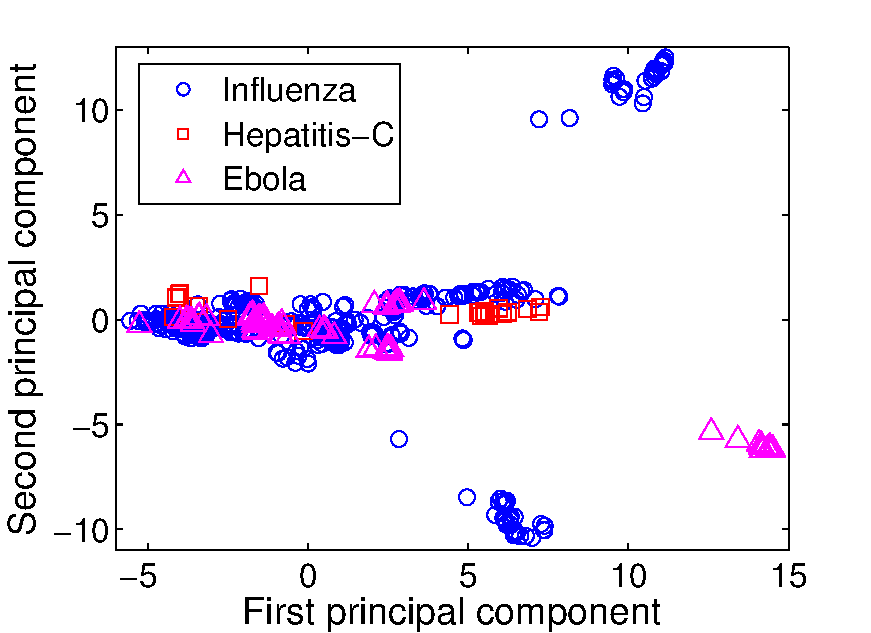
\includegraphics[scale=0.27, trim = 0 0.8cm 0 0]{figures/fig2-eps-converted-to.pdf}
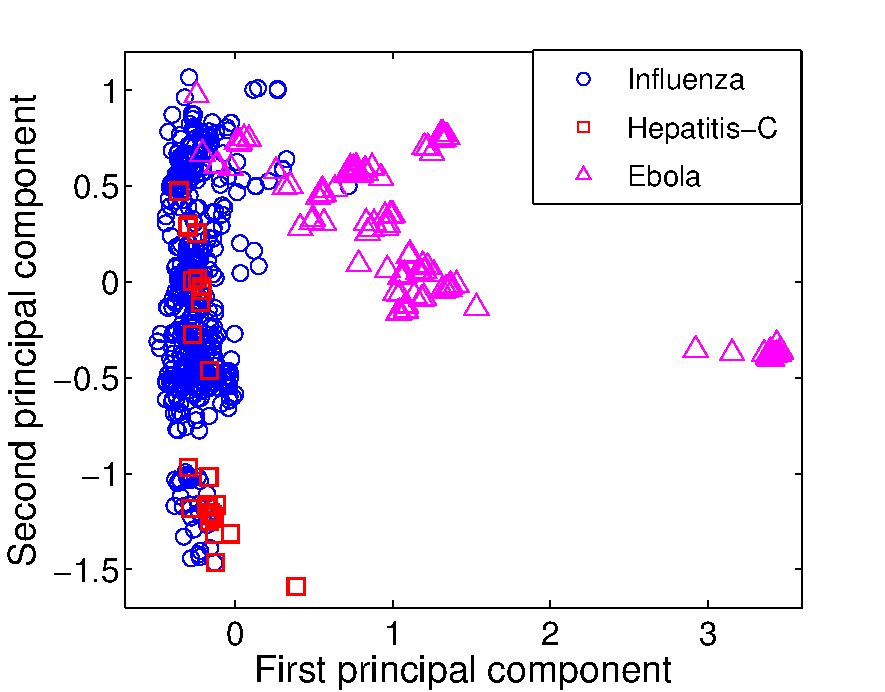
\includegraphics[scale=0.25, trim = 0 0 0 0]{figures/fig3-eps-converted-to.pdf}
}{%
\caption{Principal component analysis (PCA) of virus proteins in the original feature space (left) and the projected subspace (right). The first two principal components are shown. Shape of the points indicates which virus that protein comes from.}%
\label{fig:pca}
}
\ffigbox[0.3\columnwidth]{%
%trim option's parameter order: left bottom right top
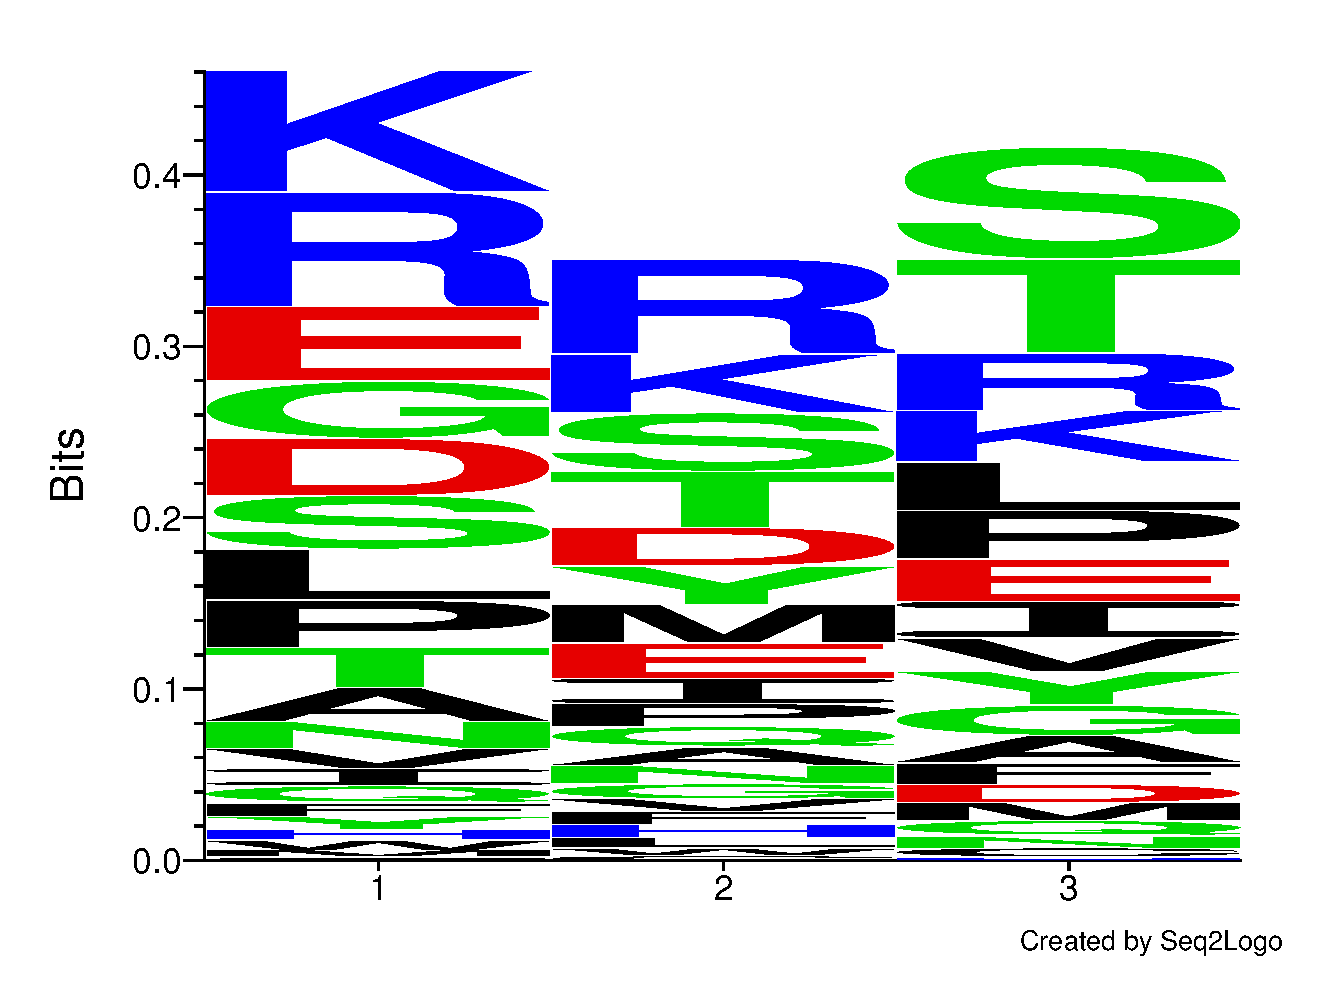
\includegraphics[scale=0.2, trim = 0 0.8cm 0 0]{figures/fig4-eps-converted-to.pdf}
}{%
\caption{Top tri-mer sequence motifs from virus proteins across all three viruses.}%
\label{fig:virus_3mer_motifs}
}
\end{floatrow}
\end{figure}

\begin{figure}[h]
\begin{floatrow}
\ffigbox[0.4\columnwidth]{%
%trim option's parameter order: left bottom right top
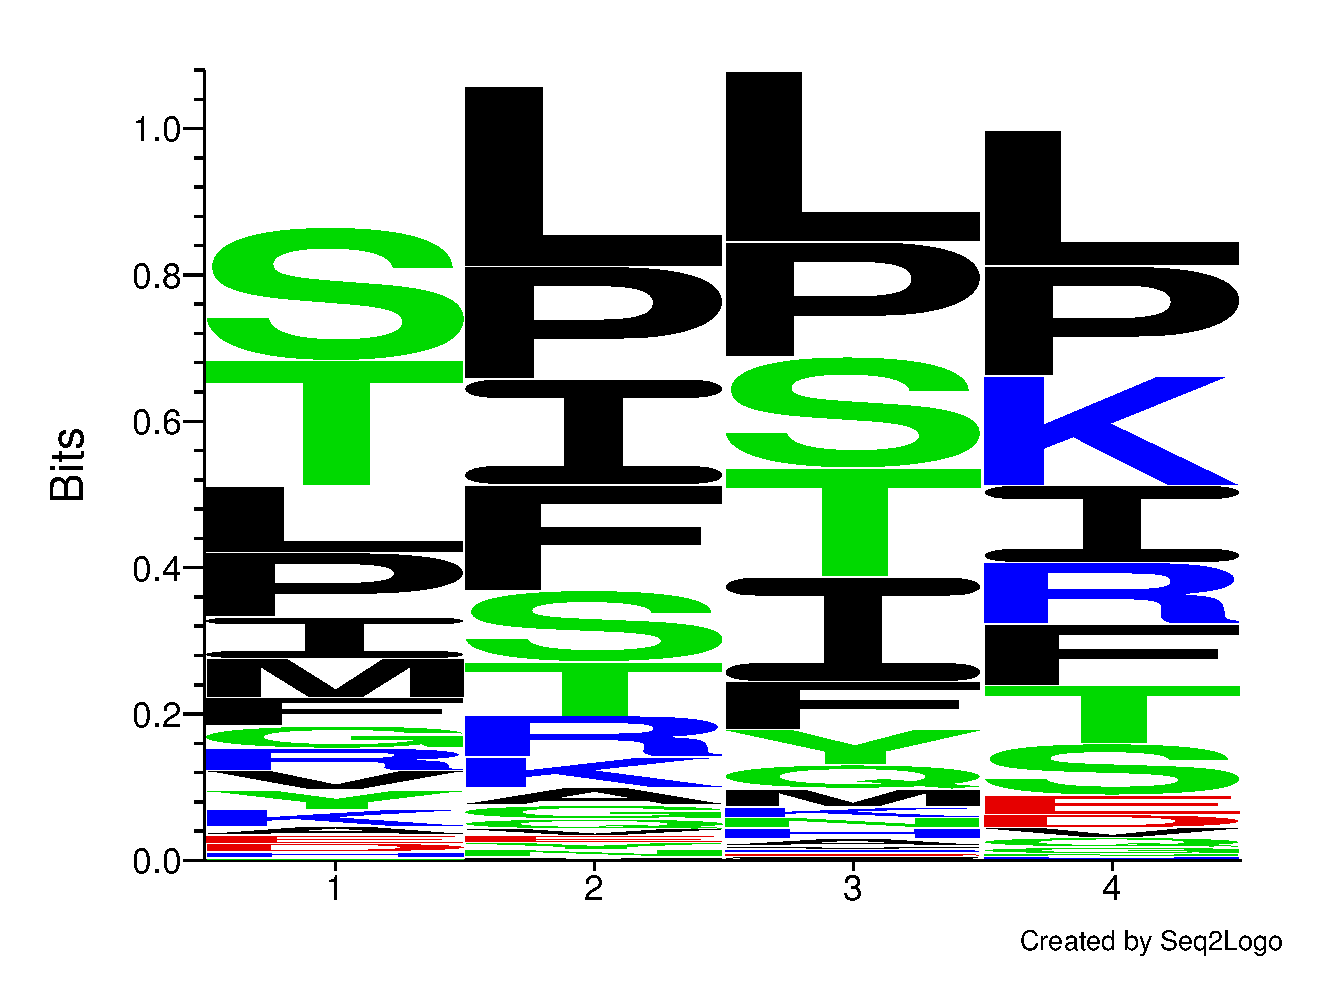
\includegraphics[scale=0.18, trim = 0 0 0 0]{figures/fig5-eps-converted-to.pdf}
}{%
\caption{Sequence motif constructed from the top four-mer features of virus proteins across all three viruses.}%
\label{fig:virus_4mer_motifs}
}
\ffigbox[0.4\columnwidth]{%
%trim option's parameter order: left bottom right top
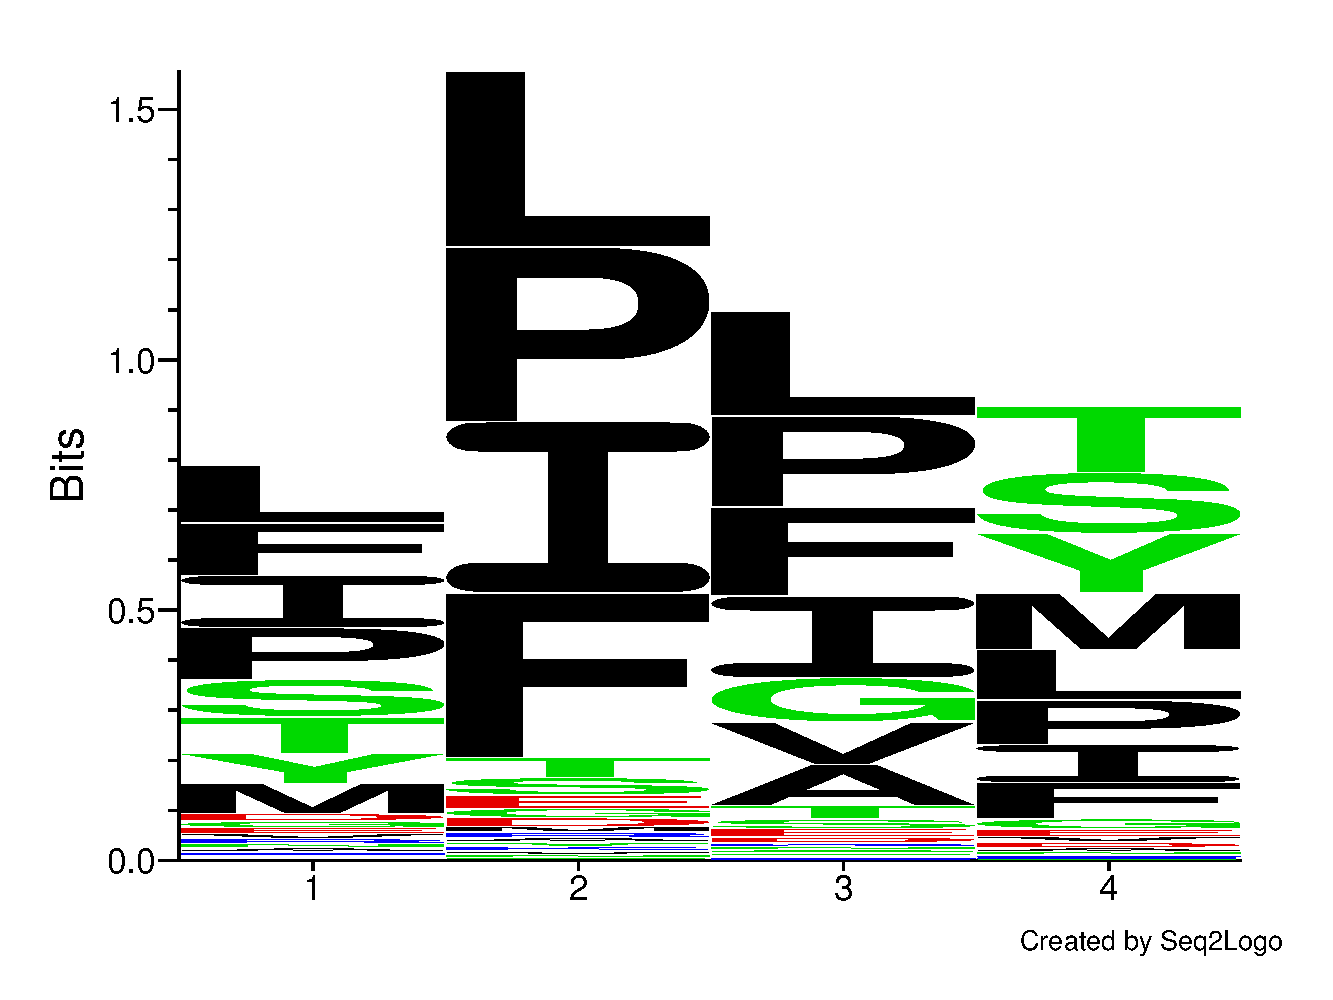
\includegraphics[scale=0.18, trim = 0 0 0 0]{figures/fig6-eps-converted-to.pdf}
}{%
\caption{Sequence motif constructed from the top four-mer features of human proteins}%
\label{fig:human_motifs}
}
\end{floatrow}
\end{figure}

\subsubsection{Sequence motifs from virus proteins}
In Figures \ref{fig:virus_3mer_motifs}-\ref{fig:human_motifs}, we show sequence motifs derived from the top $k$-mers that contribute to interactions. The significant entries of the model parameters $U$, $V$ and $\{S_t\}$ were used to 
compute these motifs. The top positive-valued entries from the product $U V^T$ indicate which pairs of features: ($(f_v, f_h)$: virus protein feature, human protein feature) are important for interactions across all the virus-human PPI tasks.
Analogously, the entries from $S_t$ give us pairs of features important to a particular virus-human task `$t$'.
We find that most of the top entries from $U V^T$ correspond to linear virus features, whereas those from the various $S_t$
involve bilinear features. We analyze the $k$-mers corresponding to the top 20 features from each of the matrices.

Note that our features do not directly correspond to a unique amino-acid $k$-mer (see Section \ref{sec:datasets}): 
the virus feature $f_v$ will map to several amino-acid sequences (for instance KKCC, KRCC, RRCC etc all map to a single feature due to the molecular similarity between the amino acids K and R being both positively charged). Given the set of top virus features we can obtain the corresponding set of 
amino-acid $k$-mers, say $AA_v$, by reversing the feature-generation step. However most of the possible $k$-mers do not appear in the 
training data (ex: out of the 160,000 (=$20^4$) possible 4-mers $\approx$24,000 appear). Let $AA_{tr}$
be the set of amino-acid k-mers that appear in the training data. Then, the intersection $I_v = AA_v \cap AA_{tr}$ gives us the important amino-acid $k$-mers from virus proteins w.r.t interaction prediction. 
To summarize $I_v$, we use a popular tool Seq2Logo \cite{seq2logo} to generate a sequence motif. 
The logos for the two-, three-, four-mers from $I_v$ are generated independently. Since we only
want to summarize, we use the Shannon logo type (which does not consider any background amino-acid distribution)
with the following settings: clustering-method=None, weight-on-prior=1 (pseudo-counts do not make sense in our
analysis). Figures \ref{fig:virus_3mer_motifs} and \ref{fig:virus_4mer_motifs} show the motif that is common across viruses. %, while the other figures highlight those motifs important in a specific species.

This procedure described above is used to analyze the most significant human protein features, obtained from
the matrix $U V^T$. These motifs are shown in Figure \ref{fig:human_motifs}. We observe that the shared tri-mer motif for virus proteins in Figure \ref{fig:virus_3mer_motifs} is dominated by 
hydrophilic amino acids (T, K, R, D, E). All other motifs seem to be dominated by hydrophobic residues (I, P, L, V, A, G)
though S and T do appear in some motifs as well.
%The human protein motifs are shown in \ref{fig:human_motifs}; the 3-mer motif show less of a pattern, in particular the first residue does not seem to have any dominant amino-acids.
%However the 4-mer seems to be dominated by hydrophobic amino-acids L, P, I, F in the first three positions and hydrophilic residues S, T, Y in the fourth.
The human protein motifs are shown in Fig \ref{fig:human_motifs}. In most cases, the first position of the tri-mer was less significant than the second and third, while for the tetramer all four positions show clear preferences.
Further analysis is in the supplementary.

\subsubsection{Novel interactions with Ebola proteins}
The top four Ebola-human PPI are all predictions for the Ebola envelope glycoprotein (GP) with four different human proteins (Note: GP is not in the gold standard PPIs). There is abundant evidence in the published literature \cite{nanbo2010} for the critical role played by GP in virus docking and fusion with the host cell.

\section{Conclusions and future extensions}
%Multitask link prediction is an important area with many applications ranging from recommendation systems to biomedical host-pathogen interactions.  
This work developed and tested a new method based on low-rank matrix completion for sharing information across tasks
%and showed significant increases in prediction performance. 
The method was evaluated in the host-pathogen protein interaction domain for three pathogens (three tasks) and exhibited significant increases in prediction accuracy. The model parameters provide several avenues for
studying host-pathogen interactions for biologists that can lead to interesting observations and insights. Finally, the model we present is general enough to be applicable on other problems such as: gene-disease relevance prediction across organisms or disease conditions. 

\scriptsize{
\bibliographystyle{plain}
%\bibliographystyle{natbib}
%\bibliographystyle{agsm}
\bibliography{references}}
%\end{scriptsize}

\end{document}
